\documentclass{article}
\usepackage{amsmath}
\usepackage{graphicx}
\usepackage{listings}
\newcommand{\includecode}[2][c]{\lstinputlisting[caption=#2, escapechar=, language=#1]{#2}}
\usepackage{minted}

\begin{document}
\lstset{language=C} 
\title{Homework 5: Feynman problem}
\author{David Jedynak}
\maketitle
\begin{abstract}
 We show how an angled tube can be created in an integer lattice gas method simulation. This angled tube is used with particle sources to perform an experiment to provide insight on the Feynman problem. The momentum transferred from the particles to the tube will be estimated to understand the response of the tube to different densities. The influence of density ratios inside and outside the tube on the force will be observed.
\end{abstract}

\section{Introduction}
The Feynman problem presents the question of what will occur when an angled tube attached to a pivot point has fluid pushed out or sucked into the tube. Will the tube rotate clockwise or counter clockwise? My prediction is that the tube will rotate clockwise when air is pushed out of the tube, if the experiment is set up as the figure below.



The Lattice Gas simulation where this experiment will be executed has constraints that particle momentum and the number of particles must be conserved. The collisions and resulting velocities can be modeled using random processes that can lower the computation cost from prior simulations that would calculate interactions between every particle based on distance, charge, mass, and fields. This can be done because the prior simulations exhibit this random behavior.


\section{Walls}
The Feynman experiment will require 2 Dimensional walls to create a right angled tube. Particles must be reflected if they hit a wall. Particles cannot pass through walls. To accomplish this requirement, velocities in different directions can be swapped. The lattice gas simulation is composed of many cells. Each cell has 9(3 by 3 grid) different values to describe particles motion in a cell.


Here are the indexes for each velocity. The value behind each index is the magnitude of the velocity in that direction
\begin{center}
Indexes ~
\begin{tabular}{l c r}
	\hline
	0 & 1 & 2 \\ \hline
	3 & 4 & 5 \\ \hline
	6 & 7 & 8 \\ 
	\hline
\end{tabular}
\end{center}

\begin{center}
Velocities corresponding to Indexes above ~
\begin{tabular}{l c r}
	\hline
	$(-v_x,+v_y)$ & $(0,+v_y)$ & $(+v_x,+v_y)$ \\ \hline
	$(-v_x,0)$ & $(0,0)$ & $(+v_x,0)$ \\ \hline
	$(-v_x,-v_y)$ & $(0,-v_y)$ & $(+v_x,-v_y)$ \\ 
	\hline
\end{tabular}
\end{center}

\subsection{Walls as Links}
A wall will be composed of links. The links will have an x and y coordinates that will be the same as the lattice cell they are interacting with. Additionally these links will also store the index of the velocity position they will be swapping. Horizontal walls will be switching [0,1,2] will be switched with [8,7,6] respectively. Vertical walls will be switching [0,3,6] will be switched with [8,5,2] respectively. Only one of these sets for each Vertical and Horizontal walls will need to be stored because both will be able to derive the second set's indexes from the first set. 
\vspace{5mm}
Code defining Horizontal Walls 
\vspace{5mm}
\begin{minted}{c}
//horizontal walls
  for (int x=x0; x<x1+1; x++){
    	links[linkcount][0] = x; //x-position
    	links[linkcount][1] = yy2;
    	links[linkcount][2] = 0;
    	linkcount++;
    	links[linkcount][0] = x; //x-position
    	links[linkcount][1] = yy2;
    	links[linkcount][2] = 1;
    	linkcount++;
    	links[linkcount][0] = x; //x-position 
    	links[linkcount][1] = yy2;
    	links[linkcount][2] = 2;
    	linkcount++;
  }
    for (int x=x1; x<x2+1; x++){
    	links[linkcount][0] = x; //x-position
    	links[linkcount][1] = yy1;
    	links[linkcount][2] = 0;
    	linkcount++;
    	links[linkcount][0] = x; //x-position
    	links[linkcount][1] = yy1;
    	links[linkcount][2] = 1;
    	linkcount++;
    	links[linkcount][0] = x; //x-position
    	links[linkcount][1] = yy1;
    	links[linkcount][2] = 2;
    	linkcount++;
  }
    for (int x=x0; x<x2+1; x++){
	links[linkcount][0] = x; //x-position
        links[linkcount][1] = yy0;
        links[linkcount][2] = 0;
        linkcount++;
        links[linkcount][0] = x; //x-position
        links[linkcount][1] = yy0;
        links[linkcount][2] = 1;
        linkcount++;
        links[linkcount][0] = x; //x-position
        links[linkcount][1] = yy0;
        links[linkcount][2] = 2;
        linkcount++;
  }
\end{minted}
\vspace{5mm}
Code Defining Vertical Walls
\vspace{5mm}
\begin{minted}{c}
  //vertical walls
if(close_tube == 1){
  for (int y=yy0; y<yy1+1; y++){
	links[linkcount][0] = x2; //x-position
	links[linkcount][1] = y;
	links[linkcount][2] = 0;
	linkcount++;
	links[linkcount][0] = x2; //x-position
	links[linkcount][1] = y;
	links[linkcount][2] = 3;
	linkcount++;
	links[linkcount][0] = x2; //x-position
	links[linkcount][1] = y;
	links[linkcount][2] = 6;
	linkcount++;
  }
}
  for (int y=yy1; y<yy2+1; y++){
	links[linkcount][0] = x1; //x-position
	links[linkcount][1] = y;
	links[linkcount][2] = 0;
	linkcount++;
	links[linkcount][0] = x1; //x-position
	links[linkcount][1] = y;
	links[linkcount][2] = 3;
	linkcount++;
	links[linkcount][0] = x1; //x-position
	links[linkcount][1] = y;
	links[linkcount][2] = 6;
	linkcount++;
  }
  for (int y=yy0; y<yy2+1; y++){
	links[linkcount][0] = x0; //x-position
	links[linkcount][1] = y;
	links[linkcount][2] = 0;
	linkcount++;
	links[linkcount][0] = x0; //x-position
	links[linkcount][1] = y;
	links[linkcount][2] = 3;
	linkcount++;
	links[linkcount][0] = x0; //x-position
	links[linkcount][1] = y;
	links[linkcount][2] = 6;
	linkcount++;
  }

\end{minted}
\vspace{5mm}
Additional code added to prevent the tube from leaking particles at several vertices.
\vspace{5mm}
\begin{minted}{c}
//2 links added to prevent leaking on the x0,yy2 and x2,yy0 squares 
	links[linkcount][0] = x0; //x-position
    	links[linkcount][1] = yy2;
    	links[linkcount][2] = 0;
    	linkcount++;
	links[linkcount][0] = x2; //x-position
    	links[linkcount][1] = yy0;
    	links[linkcount][2] = 0;
    	linkcount++;
\end{minted}

Code Defining How particles reflect off of walls (Both horizontal and vertical)
\begin{minted}{c}
void bounceback(){
  tot_vx =0;
  tot_vy =0;
  for (int lc=0; lc<linkcount; lc++){
    //quantity of partices in a given link
    int x=links[lc][0];
    int y=links[lc][1];
    //velocity of the particles in a given link
    int v=links[lc][2];
    int vx=v%3-1;
    int vy=1-v/3;
    int tmp= n[x+vx][y+vy][v];
    //summing all momemtums
    tot_vx += -2*vx*(n[x][y][8-v]-tmp);
    tot_vy += -2*vy*(n[x][y][8-v]-tmp);
    //swapping the particles trying to enter 
    //and leave to have the effect of a wall
    n[x+vx][y+vy][v]= n[x][y][8-v];
    n[x][y][8-v]=tmp;		
  }
  //measure routine stores values for plotting
  Measure();
}
\end{minted}

\section{Calculating Momentum}
 The momentum of the tube can be calculated by relating  the quantity and velocity of the particles being reflected by the tube. The momentum can be described using 2 dimensions x and y. The tube momentum in either direction will be proportional to 2 times the opposite momentum of the difference of the particles attempting to leave or enter the tube/wall. To find the total momentum, the sum of all these particle momenums will be taken over every single "link" or way particles can travel from one lattice cell to another.
 
\vspace{5mm}
$
(\rho_x,\rho_y) = -2*\sum_{link_0}^{link+1} (vel_x*(\Delta particles_x),vel_y*(\Delta particles_y))
 $
\vspace{5mm}

 Accomplishing this in the program requires a calcualting in the counceback routine previously discussed in section 2.1 to iterate through all links and make this calculation
 
 \begin{minted}{c}
    //summing all momemtums
    tot_vx += -2*vx*(n[x][y][8-v]-tmp);
    tot_vy += -2*vy*(n[x][y][8-v]-tmp);
\end{minted}
 
\section{Force as a Function of Density Ratios}

\section{Results}

\begin{figure}[H]
\centering
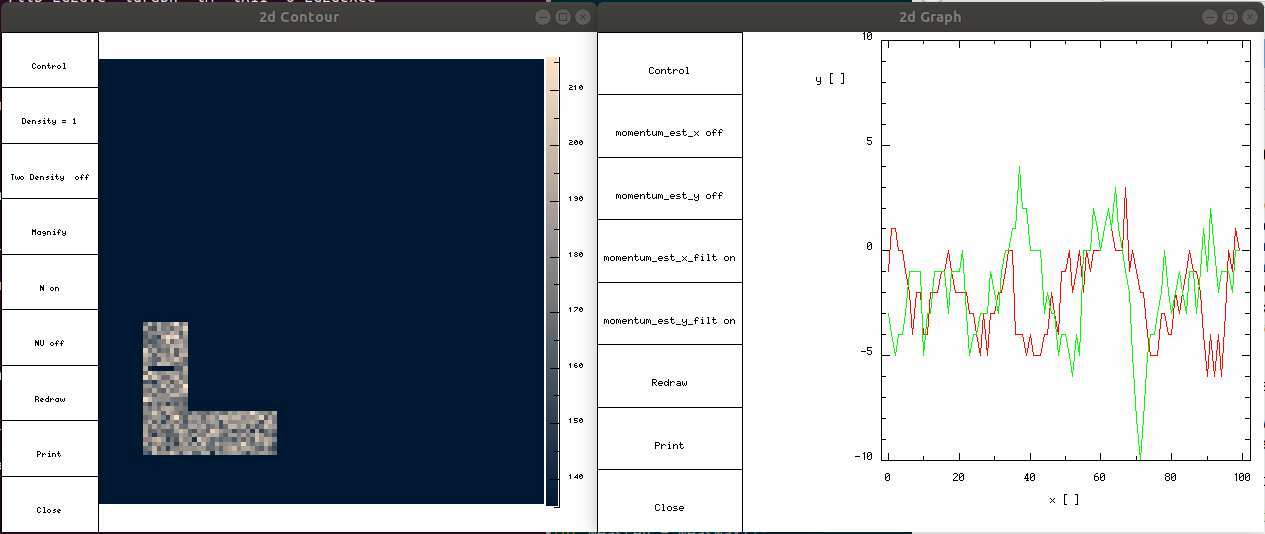
\includegraphics[scale=0.3]{p1_noleakage.png}
\caption{\label{fig} image of fully closed tube with source located inside. light color ~ high desity dark color ~low to zero density. The graph to the left shows the averaged x and y momentums centered around 0, so this is a good check that the box is sealed, beacuse otherwise there would be non zero net momentum.}
\end{figure}


\subsection{Wall}
\subsection{Calculating Momentum}
\subsection{Force as a Function of Density Ratios}



These simulations show that particles reenter at the boundaries of the simulation and that no spurious effects are obvious at the periodic boundaries.

\section{Conclusions}
In this report we have shown how to implement periodic boundary conditions in a Molecular Dynamics simulation. We have verified that our algorithm is free from obvious errors by setting up a periodic system and observing that it shows no spurious edge effects.


\appendix
\section{Code}
\lstinputlisting[language=C]{/home/david/Documents/Computational_Physics/HW5/LG2d.c}
\end{document}
  
